
\section{Spark MLLib Linear Model Class Internals}
 
RegressionModel
GeneralizedLinearModel
LinearRegressionModel
LinearRegressionWithSGD


%Ref: http://get-software.net/graphics/pgf/contrib/pgf-umlcd/pgf-umlcd-manual.pdf (not used)
%\begin{tikzpicture}
%\begin {class}[text width=8cm]{ClassName}{0 ,0}
%\attribute{name : attribute type}
%\attribute{name : attribute type = default value}
%\operation{name ( parameter list ) : type of valuereturned}
%% virtual operation
%\operation[0]{ name ( parameters list ) : type ofvalue returned}
%\end {class}
%\end {tikzpicture}

%Ref: tikzuml-v0.9.9.pdf
\begin{tikzpicture}
\begin{umlpackage } [ x=0,y=0]{ package−name}
\end{umlpackage }
\ umlemptyclass[width=15ex] { class20}
\ umlemptyclass[y=−2, width=30ex ] { class40}
\end{tikzpicture}

%Ref: http://get-software.net/graphics/pstricks/contrib/uml/uml.pdf

%Ref: http://www.texample.net/tikz/examples/tree/
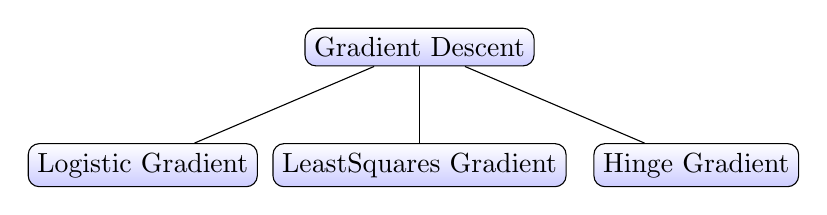
\begin{tikzpicture}[sibling distance=10em,
  every node/.style = {shape=rectangle, rounded corners,
    draw, align=center,
    top color=white, bottom color=blue!20}]]
  \node {Gradient Descent}
    child { node {Logistic Gradient} }
    child { node {LeastSquares Gradient} }
    child { node {Hinge Gradient} };
\end{tikzpicture}

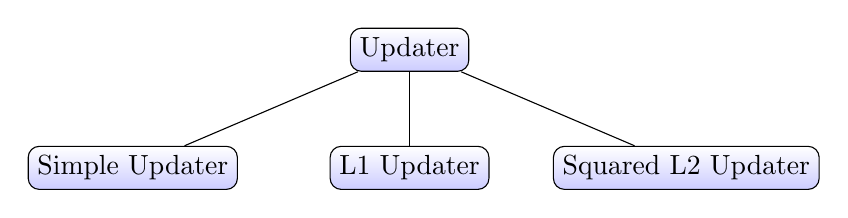
\begin{tikzpicture}[sibling distance=10em,
  every node/.style = {shape=rectangle, rounded corners,
    draw, align=center,
    top color=white, bottom color=blue!20}]]
  \node {Updater}
     child { node {Simple Updater} }
     child { node {L1 Updater} }
     child { node {Squared L2 Updater} };
\end{tikzpicture}

%Ref: UML http://ctan.imsc.res.in/graphics/pgf/contrib/pgf-umlcd/pgf-umlcd-manual.pdf

LinearRegressionWithSGD.train.run.
